\documentclass{acmart}
\usepackage{amsmath,amsfonts,amssymb,latexsym}
\usepackage{graphicx}


\title{Investigating the use of aesthetic measures over time with unsupervised evolutionary art}
\author{Ben Schlegel}
\date{\today}

\begin{abstract}
    We present a study of several aesthetic measures over time in unsupervised evolutionary art. We evolve shaders without any human evaluation, using aesthetic scores as our fitness function. We take samples of the shader at several timestamps, calculate the score, and sum all the scores up to do fitness evaluation. Included in the score is an
    additional score to reflect change in the image produced over time. We prove that interesting results can be acheived in this method, however aesthetic measures may be the wrong tool to evaluate the shaders. Results can be found at \url{https://brschlegel.github.io/EvolutionaryShaders/}
\end{abstract}
\begin{document}
\begin{titlepage}
    \maketitle
\end{titlepage}



\graphicspath{{./images/}}

\section*{Introduction}
Evolutionary art is a field investigating the use of evolutionary computing techniques to produce aesthetically pleasing images. Traditionally this involves the assistance of human judges, determining which phenotypes live on. This leads to a fitness bottleneck,
and also leads to subjectivity. Using aesthetic measures gives us numbers to look at and run statistics on, and also does not rely on humans to function. This means the production and evolution of our genotypes can be speed up massively. We have implemented three aesthetic measures to evolve our images with. The shaders will be placed on a blank canvas, and the images produced will be evaluated using a single aesthetic measure at several time steps. The sum of the scores at each time step will then be used to give a fitness score to the shader. These fitness scores will be used to determine which shaders 
survive and are used to produce the next generation.


\section*{Aesthetic Measures}
A set of X images are produced using each shader for different time steps. These are then fed through an aesthetic measurement to get a score, and the scores are then averaged to get a score for the shader. A score for producing change over time is also added, and is discussed further on. Our calculations are based on modifications of the calculations used in \textit{Investigating aesthetic measures for unsupervised evolutionary art}
\subsection*{Shannon Entropy}
Shannon entropy is an aesthetic measure that attempts to use information theory to get an aesthetic value of an image. We use a method similar to Rigau et al. [3] to calculate the score for these images. 
First we convert the image to grayscale using the average method, and then sort the image regions into a histogram of 128 values. We then calculate the score by
\begin{equation*}
    M = - \sum_{i=0}^{127} p(x_i) * log(p(x_i))
\end{equation*}
where $p(x_i)$ is the probability that a random region will have that value. The image will score high on this measure if the probability is distributed uniformly.

\subsection*{Benford Distribution}
Benford Distribution is a based on Benford's Law, which states that a list of numbers obtained in real life (Not generated) are distributed in a specific way [2]. The leading digit occurs around 30\% of the time
, the second around 18\% of the time. The distribution can be roughly modeled as 
\begin{align*}
    P(d) = log_{10}(1 + \frac{1}{d})
\end{align*}
The aesthetic measure is defined as the distance the distribution of greyscale values from the Benford distribution. To achieve this we calculate the greyscale values of each region in the image
, and then sort them into a histogram with 9 bins. We then calculate the difference by:
\begin{align*}
    d_{total} = \sum_{i=1}^9 (P(H_{image} (i)) - H_{Benford}(i)))^p
\end{align*}
Where $P(H_{image} (i))$ is the the number of entries in a bin divided by the total number of entries, and $H_{Benford}(i)$ is described by the benford distribution. Adjusting the constant $p$
results in a higher penalty for differences. In our experiments we used $p = 3$.
The aesthetic measure is then calculated using:
\begin{align*}
    M = \frac{d_{max} - d_{total}}{d_{max}}
\end{align*}
$d_{max}$ is calculated by substituting $\{1,0,0,...,0\}$ for $P(H_{image})$
\subsection*{Reflectional Symmetry}
We use a reflectional symmetry aesthetic measure similar to the one define din Heijer and Eiben. First the image is divided into 4 quadrants, $A_1$, $A_2$, $A_3$, $A_4$. Left, right top and bottom are defined as
$A_{left} = A_1 \bigcup A_3$, $A_{right} = A_2 \bigcup A_4$, $A_{top} = A_1 \bigcup A_2$, $A_{bottom} = A_3 \bigcup A_4$\\
Horizontal symmetry is defined as:
\begin{equation*}
    S_h = s(A_{left}, A_{right})
\end{equation*}
vertical symmetry is 
\begin{equation*}
    S_v = s(A_{top}, A_{bottom})
\end{equation*}
and diagonal symmetry is 
\begin{equation*}
    S_d = \frac{s(A_1, A_4) + s(A_2, A_3)}{2}
\end{equation*}
where the similarity between two areas is defined as 
\begin{equation*}
    s(A_i, A_j) = \frac{\sum^w_{x=0} \sum^h_{y=0}(sim(A_i(x,y), \bar{A_j}(x,y)))}{w*h}
\end{equation*}
where $x$ and $y$ are the coordinates of the region, and $w$ and $h$ are the width and height of the area. $\bar{A}$ is the mirrored area of $A$, with respect to the 
symmetry we are trying to measure. $sim$ is defined as
\[
    sim(A_i(x,y), A_j(x,y)) = 
    \begin{cases}
        1 & \text{if   } |A_i(x,y) - \bar{A_j}(x,y)| < \alpha\\
        0 & \text{otherwise}
    \end{cases}
\]
We use $\alpha = .05$ as our threshold.
Therefore the score for strict symmetry is 
\begin{equation*}
    M_{strict} = \frac{S_h + S_v + S_d}{3}
\end{equation*}
There is a danger, however, in just using symmetry as a fitness function, as monochrome and monotonous images are very easy to evolve, and are also very symmetrical. Heijer and Eiben point this out, and suggest
a 'liveliness' factor. We do the same here, and use our Shannon Entropy score to add some more variety to the images produced.
Therefore our score is 
\begin{equation*}
    M = M_{strict} * M_{shannon}^3
\end{equation*}

\section*{Evolutionary Algorithm}
\subsection*{Representation of shaders}
The evolution of shaders is done by our own software. In the program, shaders are represented through 3 expression trees, with one for red, blue, and green colors. In these trees, there are 
operator nodes, which have two children, and leaf nodes which do not have children. All operators have 2 children to avoid making invalid trees during mutation and crossover stages. 
Operators are split into 3 types, which determine how their children are used in calculation and writing. Type 1 operators use a "left right" orientation, for example, the plus operator: Uv.x + 3. 
Type 2 operators are functions with 2 inputs, for example the noise operator, noise(2,4). Type 3 operators are functions with only one input, and to preserve each operator having 2 children, for example the PlusCos operator: 3 + cos(14).
\\
\begin{tabular}{|c|c|c|c|}
    \hline
    Operator & Type&  Example & Description\\
    \hline
    Plus & 1 & Uv.x + 32 & Standard Addition \\
    \hline
    Minus & 1 &TIME - 3 & Standard Subtraction \\
    \hline
    Multiply & 1 & 15 * Uv.y & Standard Multiplication  \\
    \hline
    Divide & 1 & 23 /32 & Standard Division  \\
    \hline
    PlusCos & 3 & Uv.y Cos(34) & Left child added to cosine of right child  \\
    \hline
    MultCos & 3 & 20 * Cos(Uv.x) & Left child multiplied by cosine of right child  \\
    \hline
    PlusSin & 3  & 24 + sin(32) & Left child added to sin of right child  \\
    \hline
    Multiply & 3 & 15 * sin(21)& Left child multiplied by sine of right child   \\
    \hline
    Impulse & 2 & impulse(2,4) & Shaping function with peak then smooth die-off. \\ & & & Left child stretches function, right child is input\\
    \hline
    Parabola & 2 & parabola(2,3) & Shaping function that turns interval (0,1) to parabola \\
    & & & Left child stretches, right child is input\\
    \hline
\end{tabular}\\\\
Leaf nodes are further split into constants, and variables. 
\\\\
\begin{tabular}{|c|c|}
    \hline
    Variable & Description \\ 
    \hline
    Uv.x & x coordinate of current pixel, normalized [0,1]\\
    \hline
    Uv.y & y coordinate of current pixel, normalized [0,1]\\
    \hline
    TIME & Time since shader started\\
    \hline
\end{tabular}\\\\
These expression trees are traversed inorder to write the trees into a Godot shader. The shader's trees are solved to produce a matrix of colors at different time steps. The average difference between every timestep and its following timestep is then computed,
and then the average of those averages is added to the fitness score, with shdaders that vary more being favored over more static shaders.
\subsection*{Evolving shaders}
To start, the algorithm is initialized by shaders with random numbers of nodes and randomized values. Then each shader has its fitness score assigned, by the average difference over time and the chosen aesthetic measure. 
After the shaders have had their fitness value calculated X number of survivors are selected. The survivors are then paired up, and crossed over by swapping 2 nodes (and by extension its children) on each red, blue, and green
tree. Then Y copies are made of each survivor, and then mutated. Then the procedure is repeated until desired stopping point.
\subsection*{Experiments}
For our experiments each measure was given 300 generations, with a population size of 400 and 50 survivors, with the exception of Benford, which was done with 150 generations and a population of 200. Fitness scores were given by summing up the aesthetic measure scores for each timestep.
We used 20 timesteps, and for calculating the aesthetic measure scores we used 1600 regions in a 40 x 40 grid. Survivors were chosen, paired up, and crossed over. The product of this 
cross over were used to create the new population by mutation. Each tree in the shader were limited to 20 leaves to avoid bloating of computation time.

\newpage
\section*{Results}
We encourage anyone interested in the results to see the shaders at: \url{https://brschlegel.github.io/EvolutionaryShaders/}, as they cannot be shown animating here.
\subsection*{Shannon's Entropy}
\begin{figure}[h!]
\caption{Survivors of Shannon's Entropy measure at time = 0 seconds}
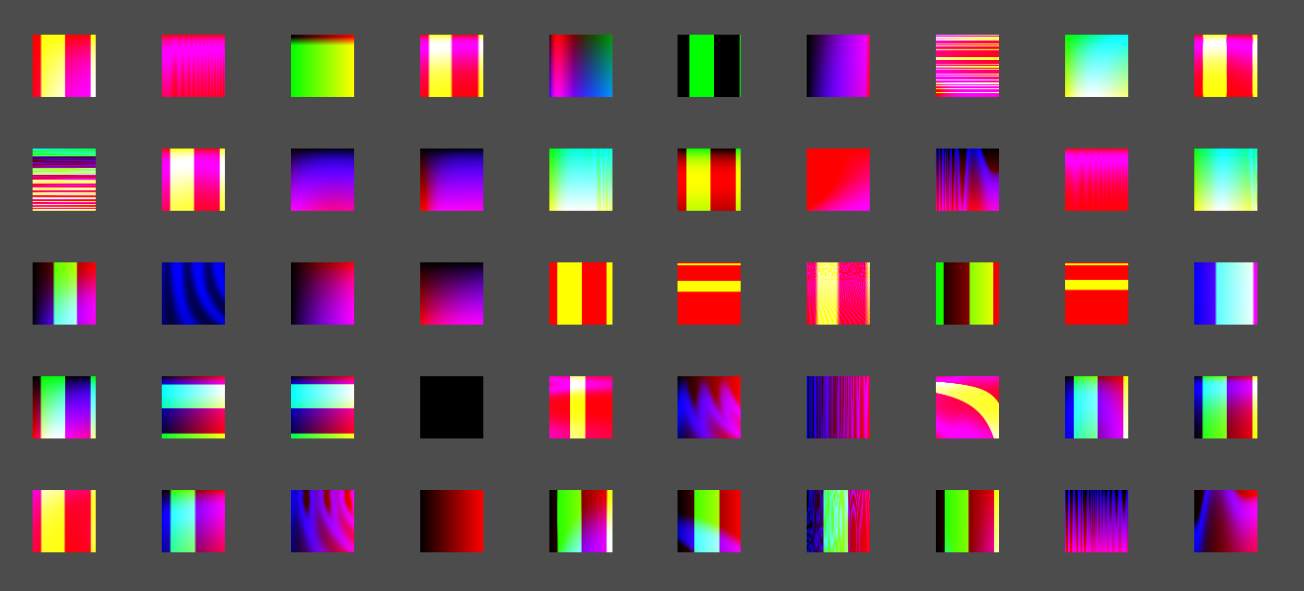
\includegraphics[width =\textwidth]{Shannon_0.PNG}
\end{figure}

This aesthetic measure looked for a uniform distribution of the grayscale values of the pixels. In some cases this seems to have been successful, and we see nice gradients forming.
In others, the effects seems to have been lost, paticularly with the bars that this measures seem to encourage often have very sharp lines. Perhaps most interestingly were the shaders that
seem to follow the bar pattern, but upon closer inspection one can see the soft gradient in the background that gives rise to a nice uniformly distributed greyscale values.

\begin{figure}[h!]
\caption{Survivors of Shannon's Entropy measure at time = 5 seconds}
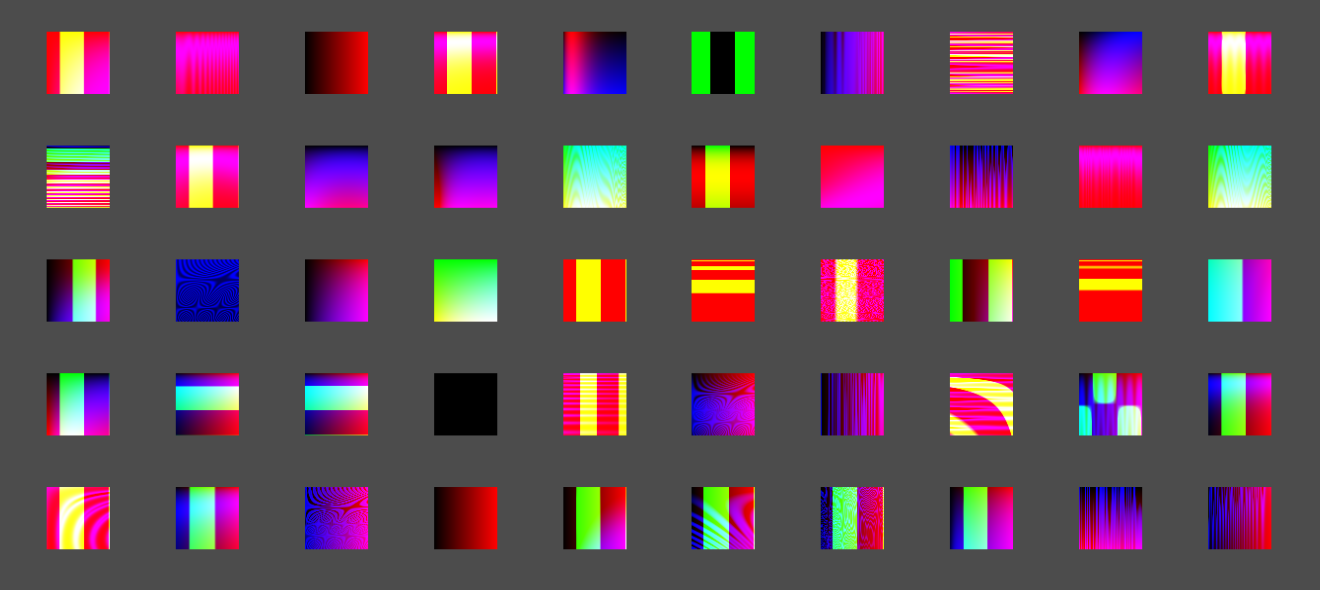
\includegraphics[width = \textwidth]{Shannon_5.PNG}
\end{figure}
Almost all the shaders produced by this measure have some sort of large movement/change happening over time. While many shaders have very cyclical changes, those that 
have changes that don't repeat always tend to add more detail to the image and either increase the number of discernible shapes/objects, or add so many objects that they begin to lose shape.
As this leads to a more uniform grayscale distribution, this makes sense.

\subsection*{Benford's Distribution}
\begin{figure}[h!]
    \caption{Survivors of Benford Distribution measure at time = 0 seconds}
    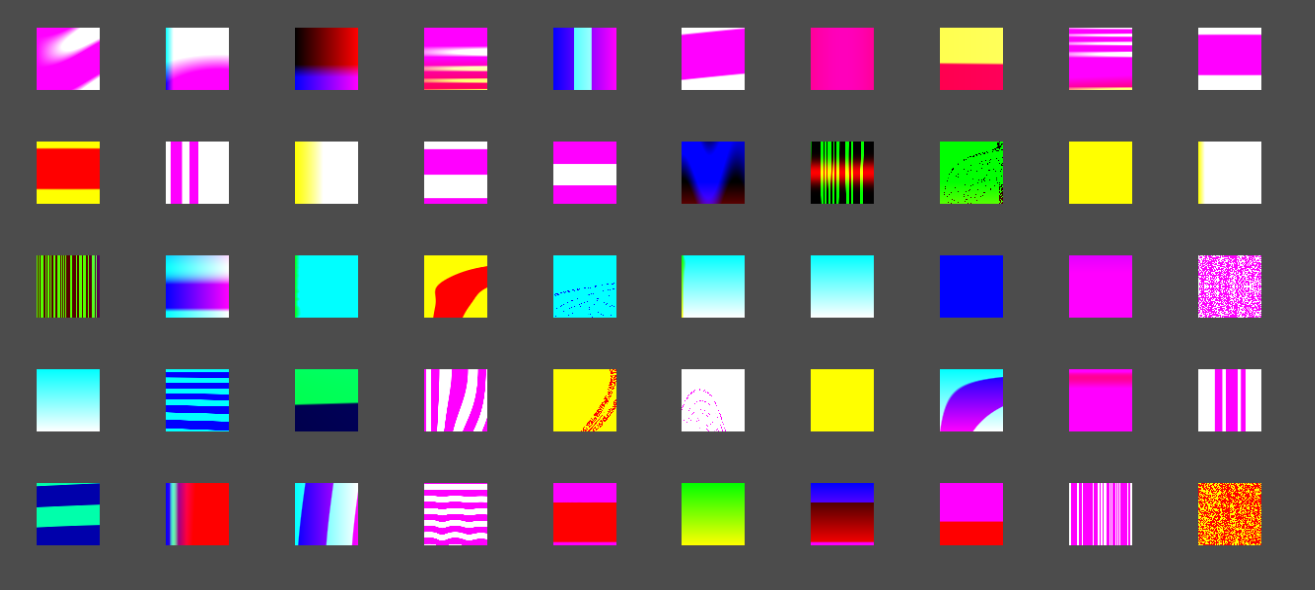
\includegraphics[width =\textwidth]{Benford_0.PNG}
\end{figure}
With the Benford Distribution measure, we expected to see lots of dark colors with smaller amounts of lighter colors, but that's not really what we see, at least at first. Many of the images
do seem to have some interesting distributions in greyscale value, but there's alot more white than one would expect. We see some more of the bar pattern from earlier, but there is certainly more deviation from it in this pattern,
as well as much more chaos/complexity in the images themselves.
\newpage
\begin{figure}[h!]
    \caption{Survivors of Benford Distribution measure at time = 5 seconds}
    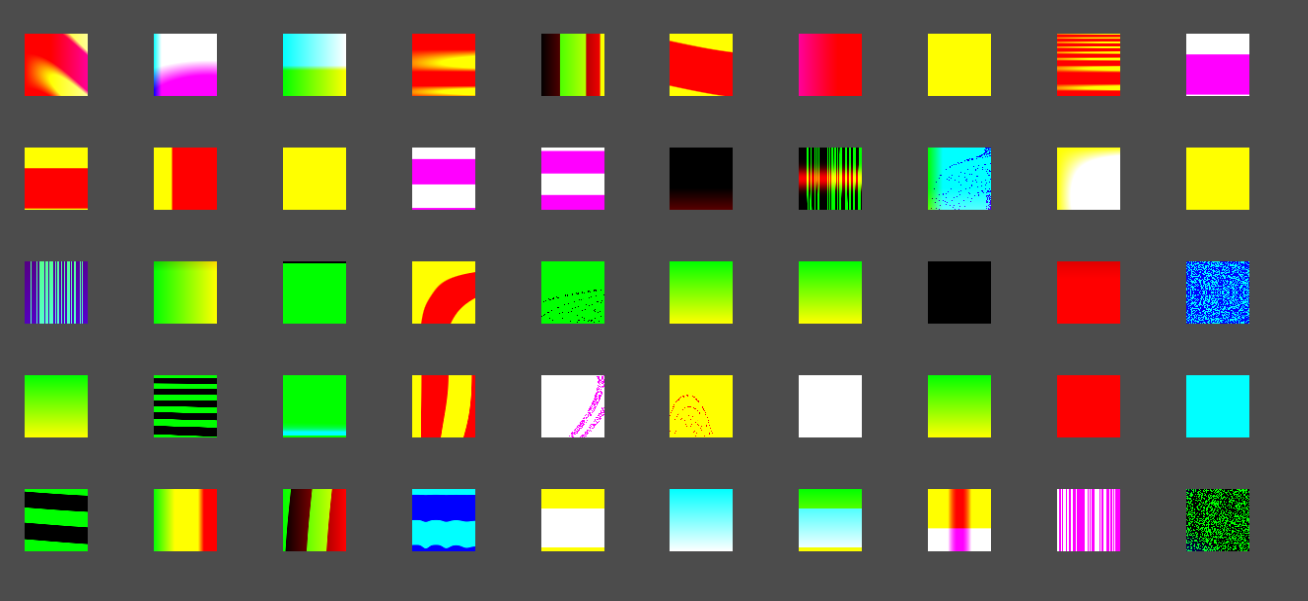
\includegraphics[width =\textwidth]{Benford_5.PNG}
\end{figure}
Over the passage of time, the colors in most of the images flip flop between dark and green, and bright and blue. This oscillating green tree is likely what allowed images with
alot of white to score highly on the measure. If a final mutation took this oscillating green value out of the equation, shaders with alot of white would survive on if competetion was limited enough or the 
mutation was easy enough to make.

\subsection*{Reflectional Symmetry}

\begin{figure}[h!]
    \caption{Survivors of Reflectional Symmetry measure at time = 0 seconds}
    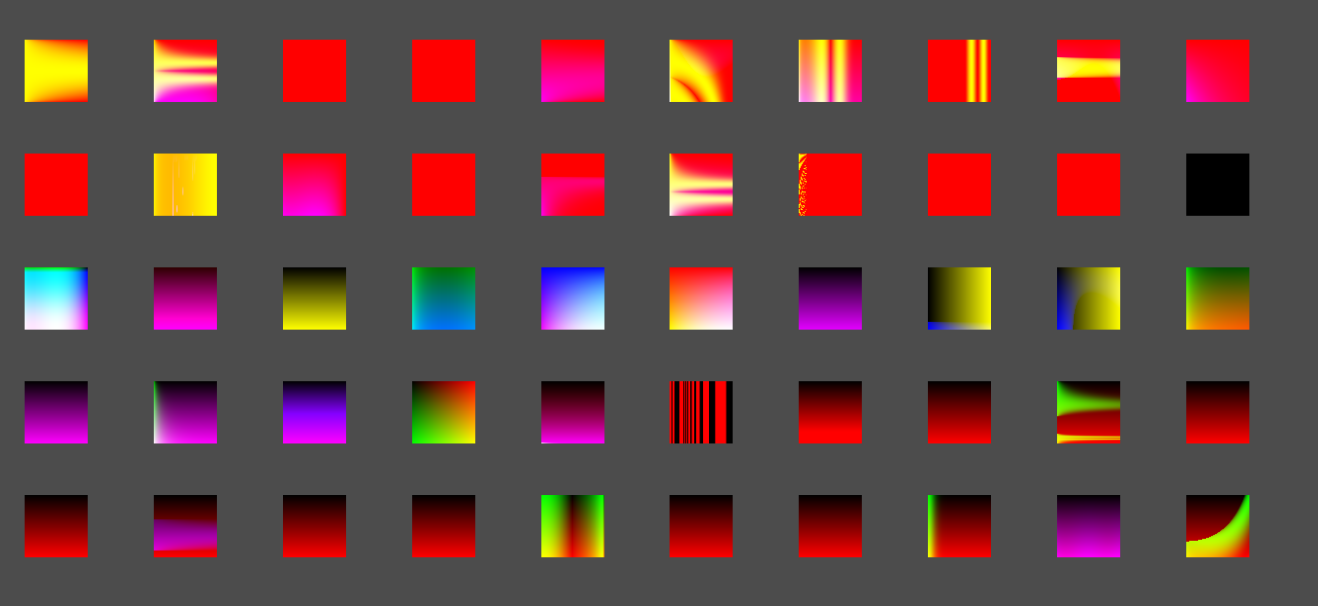
\includegraphics[width =\textwidth]{Reflectional_0.PNG}
\end{figure}
While many of the shaders evolved here did have lots of reflectional symmetry, our goal of producing interesting images seems to have been largely incomplete. The magnitudes of the 
shannon entropy score were lower than the magnitudes of the reflectional symmetry score, making it difficult to balance the two to produce interesting images that were still symmetrical. 
The existence of several interesting shaders in the surviving group seems to show that getting better results may have been possible with the current set up, if the algorithm had more time to search.
Of note, those images that were somewhat successful in our goals only satisfied one or two of our symmetries, never all of them, and only ever satisfied one with precision.

\begin{figure}[h!]
    \caption{Survivors of Reflectional Symmetry measure at time = 5 seconds}
    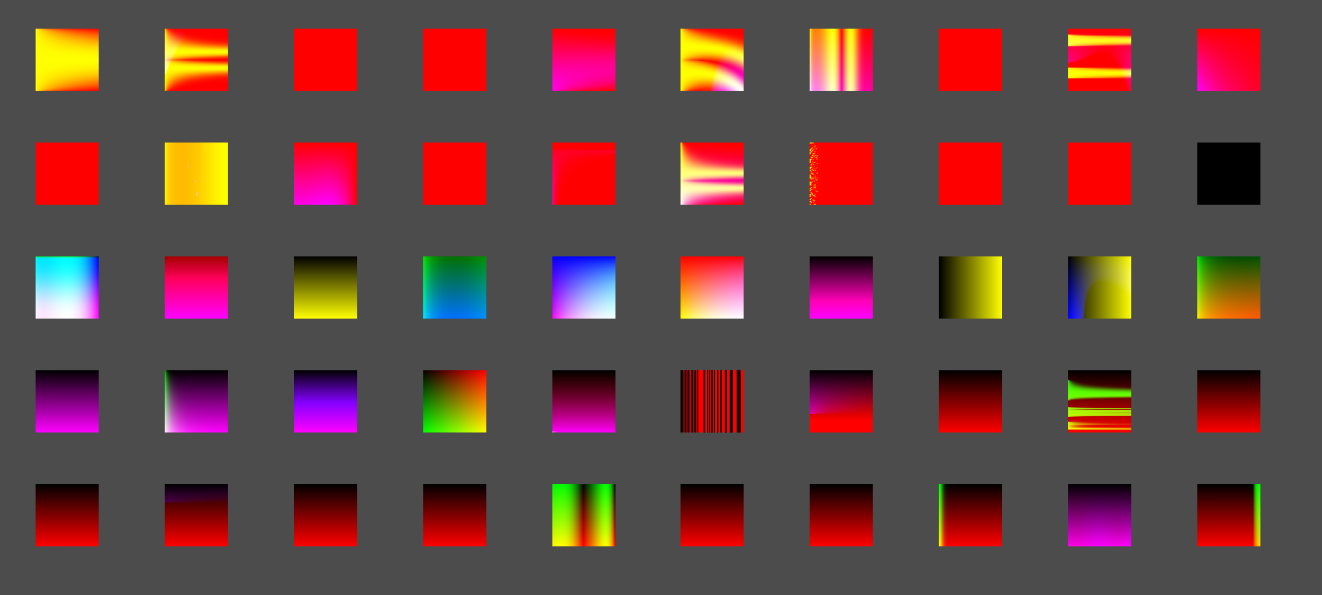
\includegraphics[width =\textwidth]{Reflectional_5.PNG}
\end{figure}
This measure also had the least relative change over time in comparison to the other measures in these expreriments. While a different scaling number was used to augment the change over time in an 
attempt to consolidate the difference in score magnitude, increasing the scaling number too much would result in a breakdown of symmetry.

\section*{Discussion of Overall Results}
Results seemed middling at best. The shaders produced seemed to hint at the measures rather than fully embody them. There are several factors that could contribute to this.
\subsection*{The Phenotype}
The phenotype for these shaders were 3 expression trees. Mutation on these trees is very volatile, as any mutation has its effect rippled up the tree. Each tree was mutated between 3-5 times in each generation, which may have 
proved to be too much. In addition, for any color other than white or black, the value of at least one tree when solved must come between 0 and 1, which is a high level of precision, especially when there is a cap on 
the number of leaves in a tree. While many of the shaders proved this was possible and had many varying colors, its possible that many shaders were thrown out due to this fact. You can also see in Figures 1-4
monochrome or close to monochrome shaders, which would have scored poorly on these measures. This could imply that monochrome shaders were very plentiful each generation, and due to that they were able to survive. This could also mean 
that it was very easy for an interesting shader to mutate into a monochrome one. Finally, these measures dealt with region values, made to approximate pixel values, while the phenotype
was using equations to color the pixels in a texture. The seperation between what we are measuring and how we are generating new shaders may make the measure hard to approximate by our algorithm.
In the future, it may prove helpful to allow the survivors to continue unchanged/mutated to the next generation, so that high scoring shaders aren't wiped out by volatile mutations.

\subsection*{Difference over time}
Part of the motivation for using shaders to create the images we see was to explore the use of aesthetic measures over time. To ensure that the shaders actually utilized this
an average diffence, scaled by a constant was added to each measures score. This now meant however that shaders were trying to accomplish two things at once, satisfy the measure at all 
timesteps, as well as produce enough change. Managing the scaling factor also proved difficult, especially because each measure had a different magnitude in its score. A way around this could be
making the average difference over time be a threshold, with shaders falling below a certain value having a score of 0.


\subsection*{Computational Restrictions}
While the program was multithreaded to increase computation speed, all calculations were still done on the CPU. Using one or multiple GPUs would have allowed for far more generations. It also may have 
helped solve the difference over time problem, as maybe given enough time shaders could have gotten close enough to the max scores of their measures that they need to get higher scores on the difference over time metric to compete.
That being said, the shaders did seem to reach a sort of optimum for the environment they were in, with the exception of possibly Reflectional Symmetry. The graphs of their average score 
are seen below: 

\begin{figure}[h!]
    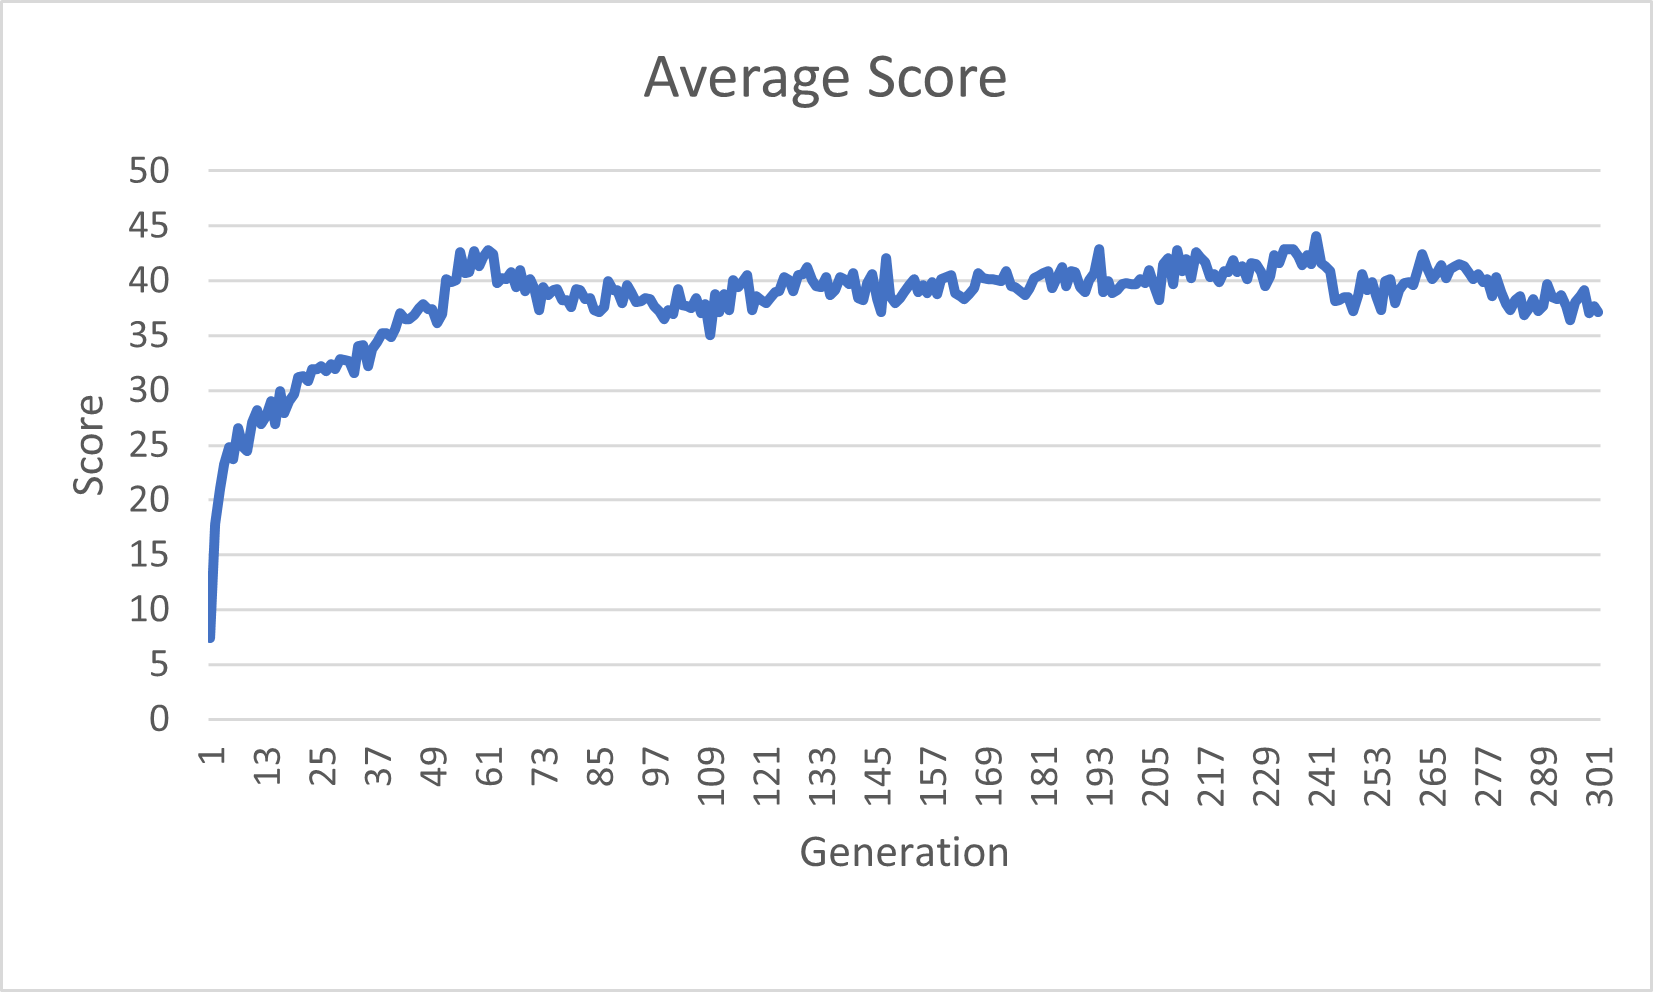
\includegraphics[width =\textwidth]{Shannon_AvgScoreGen.png}
\end{figure}

\begin{figure}[h!]
    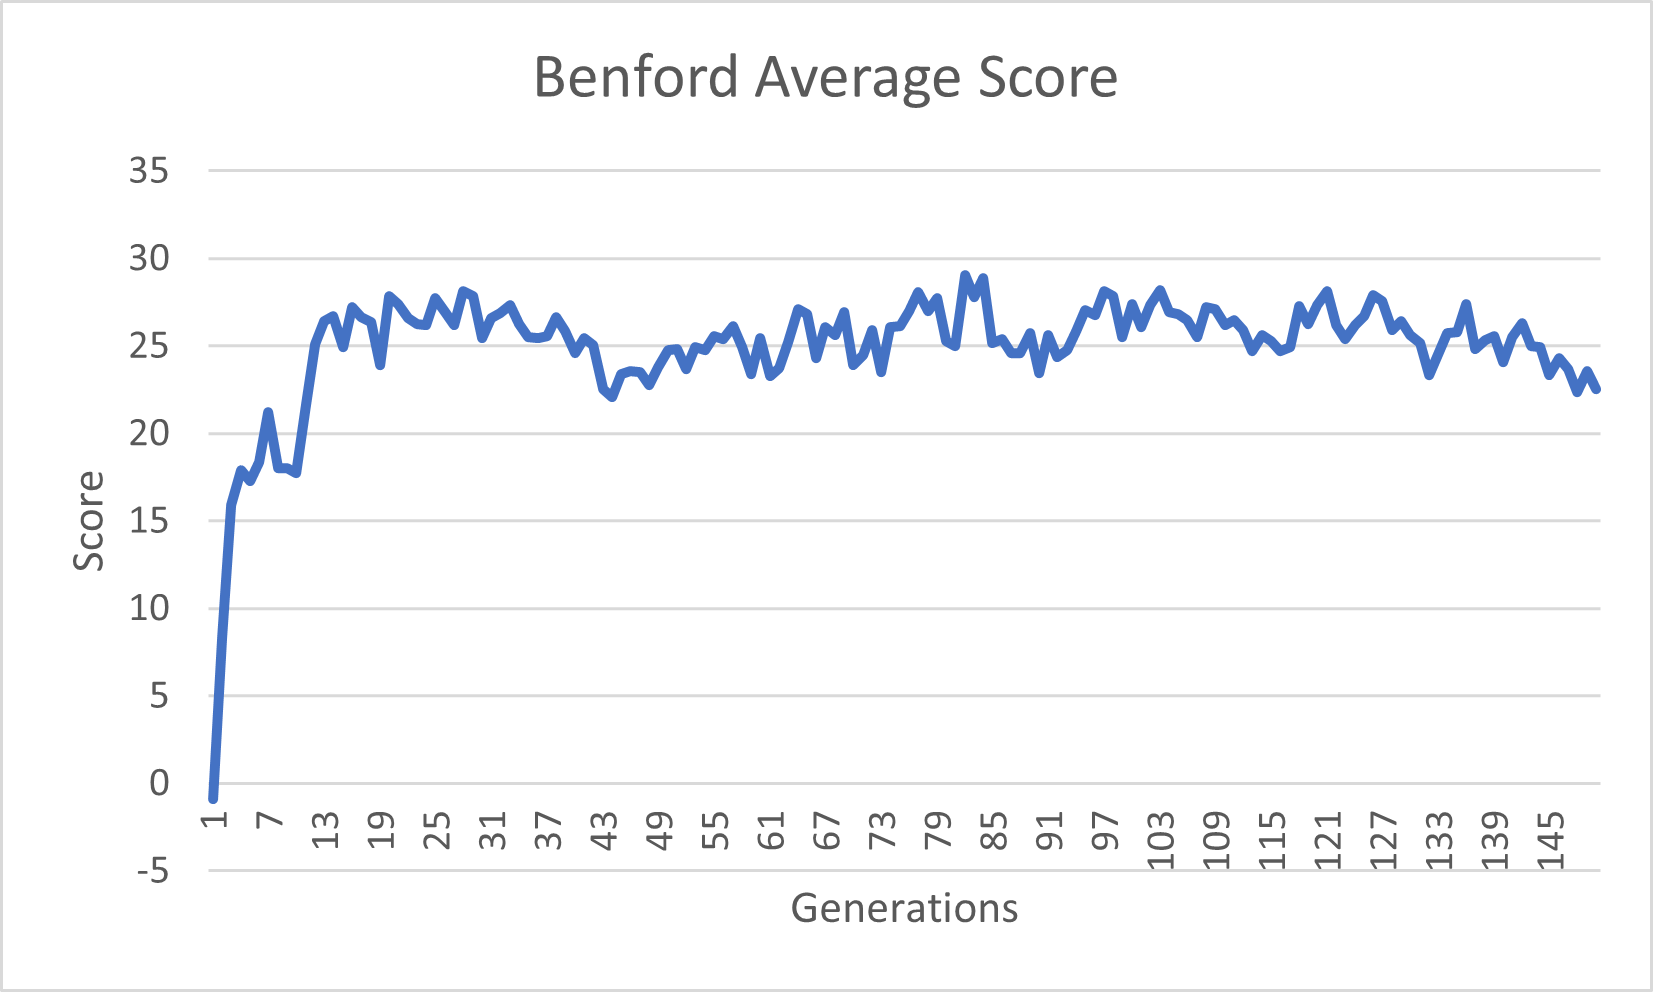
\includegraphics[width =\textwidth]{Benford_AvgScoreGen.png}
\end{figure}

\begin{figure}[h!]
    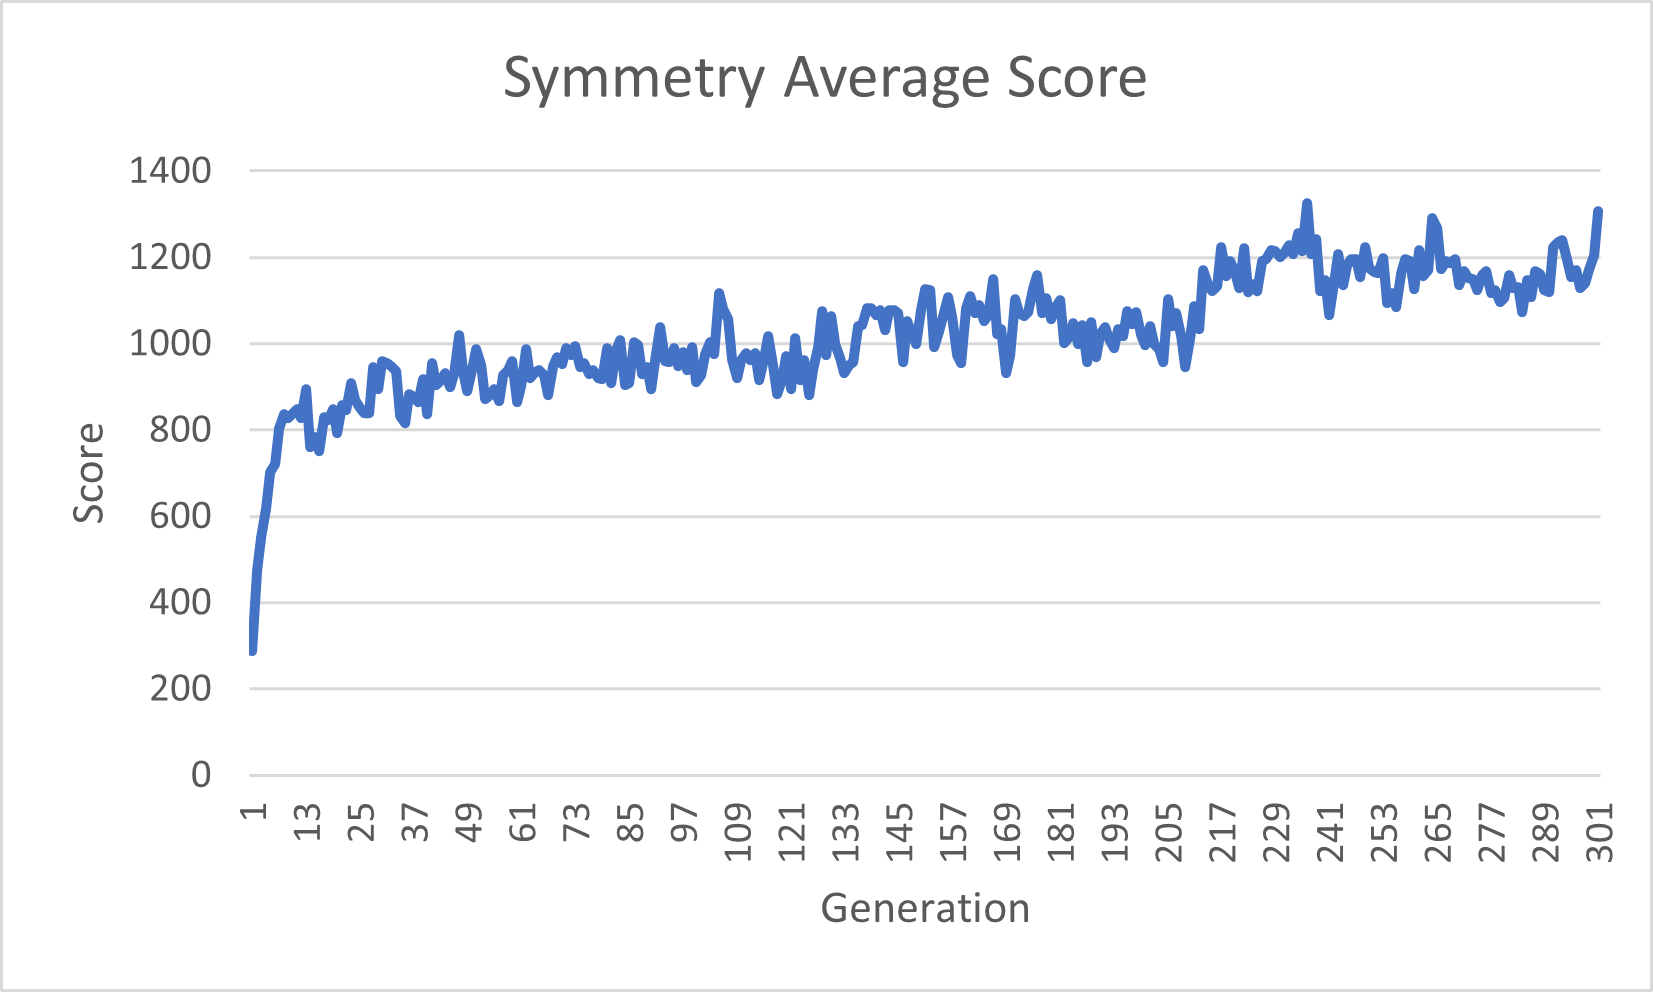
\includegraphics[width =\textwidth]{Symmetry_AvgScoreGen.png}
\end{figure}

\section*{Conclusions}
In this paper we have investigated the using of a shading language for generating images to satisfy aesthetic measures as well as change over time. We found results to be rather mild, 
especially when concerning aesthetic measures. Future work could in making aesthetic measures more suited for this method of generating images, or pivoting to working with the its strengths, such
as evolving for differences over time alone. Overall we have proven that expression trees can be evolved to produce unique images, even if those images aren't particularly well suited for 
the aesthetic measures chosen.

\begin{thebibliography}{9}

    \bibitem{BigPaper}
    Eelco den Heijer, A.E. Eiben,
    \textit{Investigating aesthetic measures for unsupervised evolutionary art}, in
    Swarm and Evolutionary Computation,
    Volume 16,
    2014,
    Pages 52-68,

    \bibitem{Benfords} 
    E. del Acebo, M. Sbert, \textit{Benford's law for natural and synthetic images}, in: 
    L. Neumann et al. (Ed.), Computational Aesthetics 2005, Eurographics Association, 2005.. 
    , pp. 169–176.
    
    \bibitem{Shannon } 
    J. Rigau, M. Feixas, M. Sbert
    \textit{Informational aesthetics measures}
    IEEE Comput. Graph. Appl., 28 (2) (2008), pp. 24-34

    \end{thebibliography}
\end{document}